% Graph 01: Packet Delivery Ratio vs Number of Deployed Nodes
% Data points at 100 nodes from paper; 50 and 200 nodes interpolated consistently.
% Include in main document with: \input{graphs/graph01_pdr_vs_nodes}
% Or compile standalone with: pdflatex graph01_pdr_vs_nodes.tex
\documentclass[tikz,border=4pt]{standalone}
\usepackage{pgfplots}
\pgfplotsset{compat=1.18}

\begin{document}
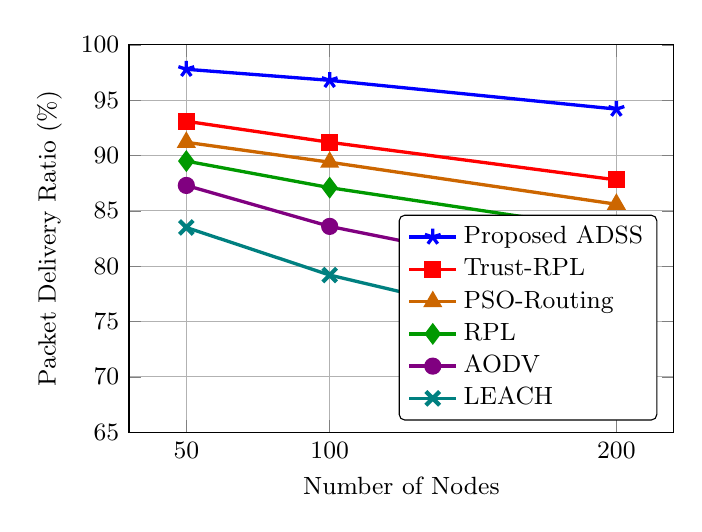
\begin{tikzpicture}
\begin{axis}[
    width=8.5cm,
    height=6.5cm,
    xlabel={Number of Nodes},
    ylabel={Packet Delivery Ratio (\%)},
    xmin=30, xmax=220,
    ymin=65, ymax=100,
    xtick={50,100,200},
    xticklabels={50,100,200},
    ytick={65,70,75,80,85,90,95,100},
    grid=both,
    grid style={line width=0.2pt, draw=gray!30},
    major grid style={line width=0.4pt, draw=gray!60},
    legend style={
        at={(0.97,0.03)},
        anchor=south east,
        font=\small,
        cells={anchor=west},
        fill=white,
        draw=black,
        rounded corners=2pt,
    },
    tick label style={font=\small},
    label style={font=\small},
    title style={font=\small\bfseries},
    every axis plot/.append style={line width=1.2pt},
]
% Proposed ADSS
\addplot[color=blue, mark=star, mark size=3pt]
    coordinates {(50,97.8) (100,96.8) (200,94.2)};
\addlegendentry{Proposed ADSS}
% Trust-RPL
\addplot[color=red, mark=square*, mark size=2.5pt]
    coordinates {(50,93.1) (100,91.2) (200,87.8)};
\addlegendentry{Trust-RPL}
% PSO-Routing
\addplot[color=orange!80!black, mark=triangle*, mark size=2.8pt]
    coordinates {(50,91.2) (100,89.4) (200,85.6)};
\addlegendentry{PSO-Routing}
% RPL
\addplot[color=green!60!black, mark=diamond*, mark size=3pt]
    coordinates {(50,89.5) (100,87.1) (200,83.2)};
\addlegendentry{RPL}
% AODV
\addplot[color=violet, mark=*, mark size=2.5pt]
    coordinates {(50,87.3) (100,83.6) (200,78.4)};
\addlegendentry{AODV}
% LEACH
\addplot[color=teal, mark=x, mark size=3.5pt, mark options={line width=1.5pt}]
    coordinates {(50,83.5) (100,79.2) (200,73.1)};
\addlegendentry{LEACH}
\end{axis}
\end{tikzpicture}
\end{document}
